%
\documentclass[10pt,a4paper]{article}


\usepackage{array}
\usepackage{subfigure}
\usepackage{graphicx}
\usepackage{amssymb}
\usepackage{amsmath}
\usepackage{cite}
\usepackage{color}
\usepackage{url}
\usepackage[lined,linesnumbered,ruled,norelsize]{algorithm2e}
\usepackage{listings}
\lstset{
  language=Octave, 
  basicstyle=\footnotesize, 
  frame=single, 
  showspaces=false, 
  showstringspaces=false}
\date{}




\begin{document}

\title{Technical Report 7: Non-Linear SVM Classification with Kernels}

\maketitle

The SVM classifier is trained by RBF kernel in LIBSVM. We take different values of $\gamma$, and report the results as follows.
%
%
    \begin{figure}[htb!]
       \begin{center}
       \parbox{.45\columnwidth}{\center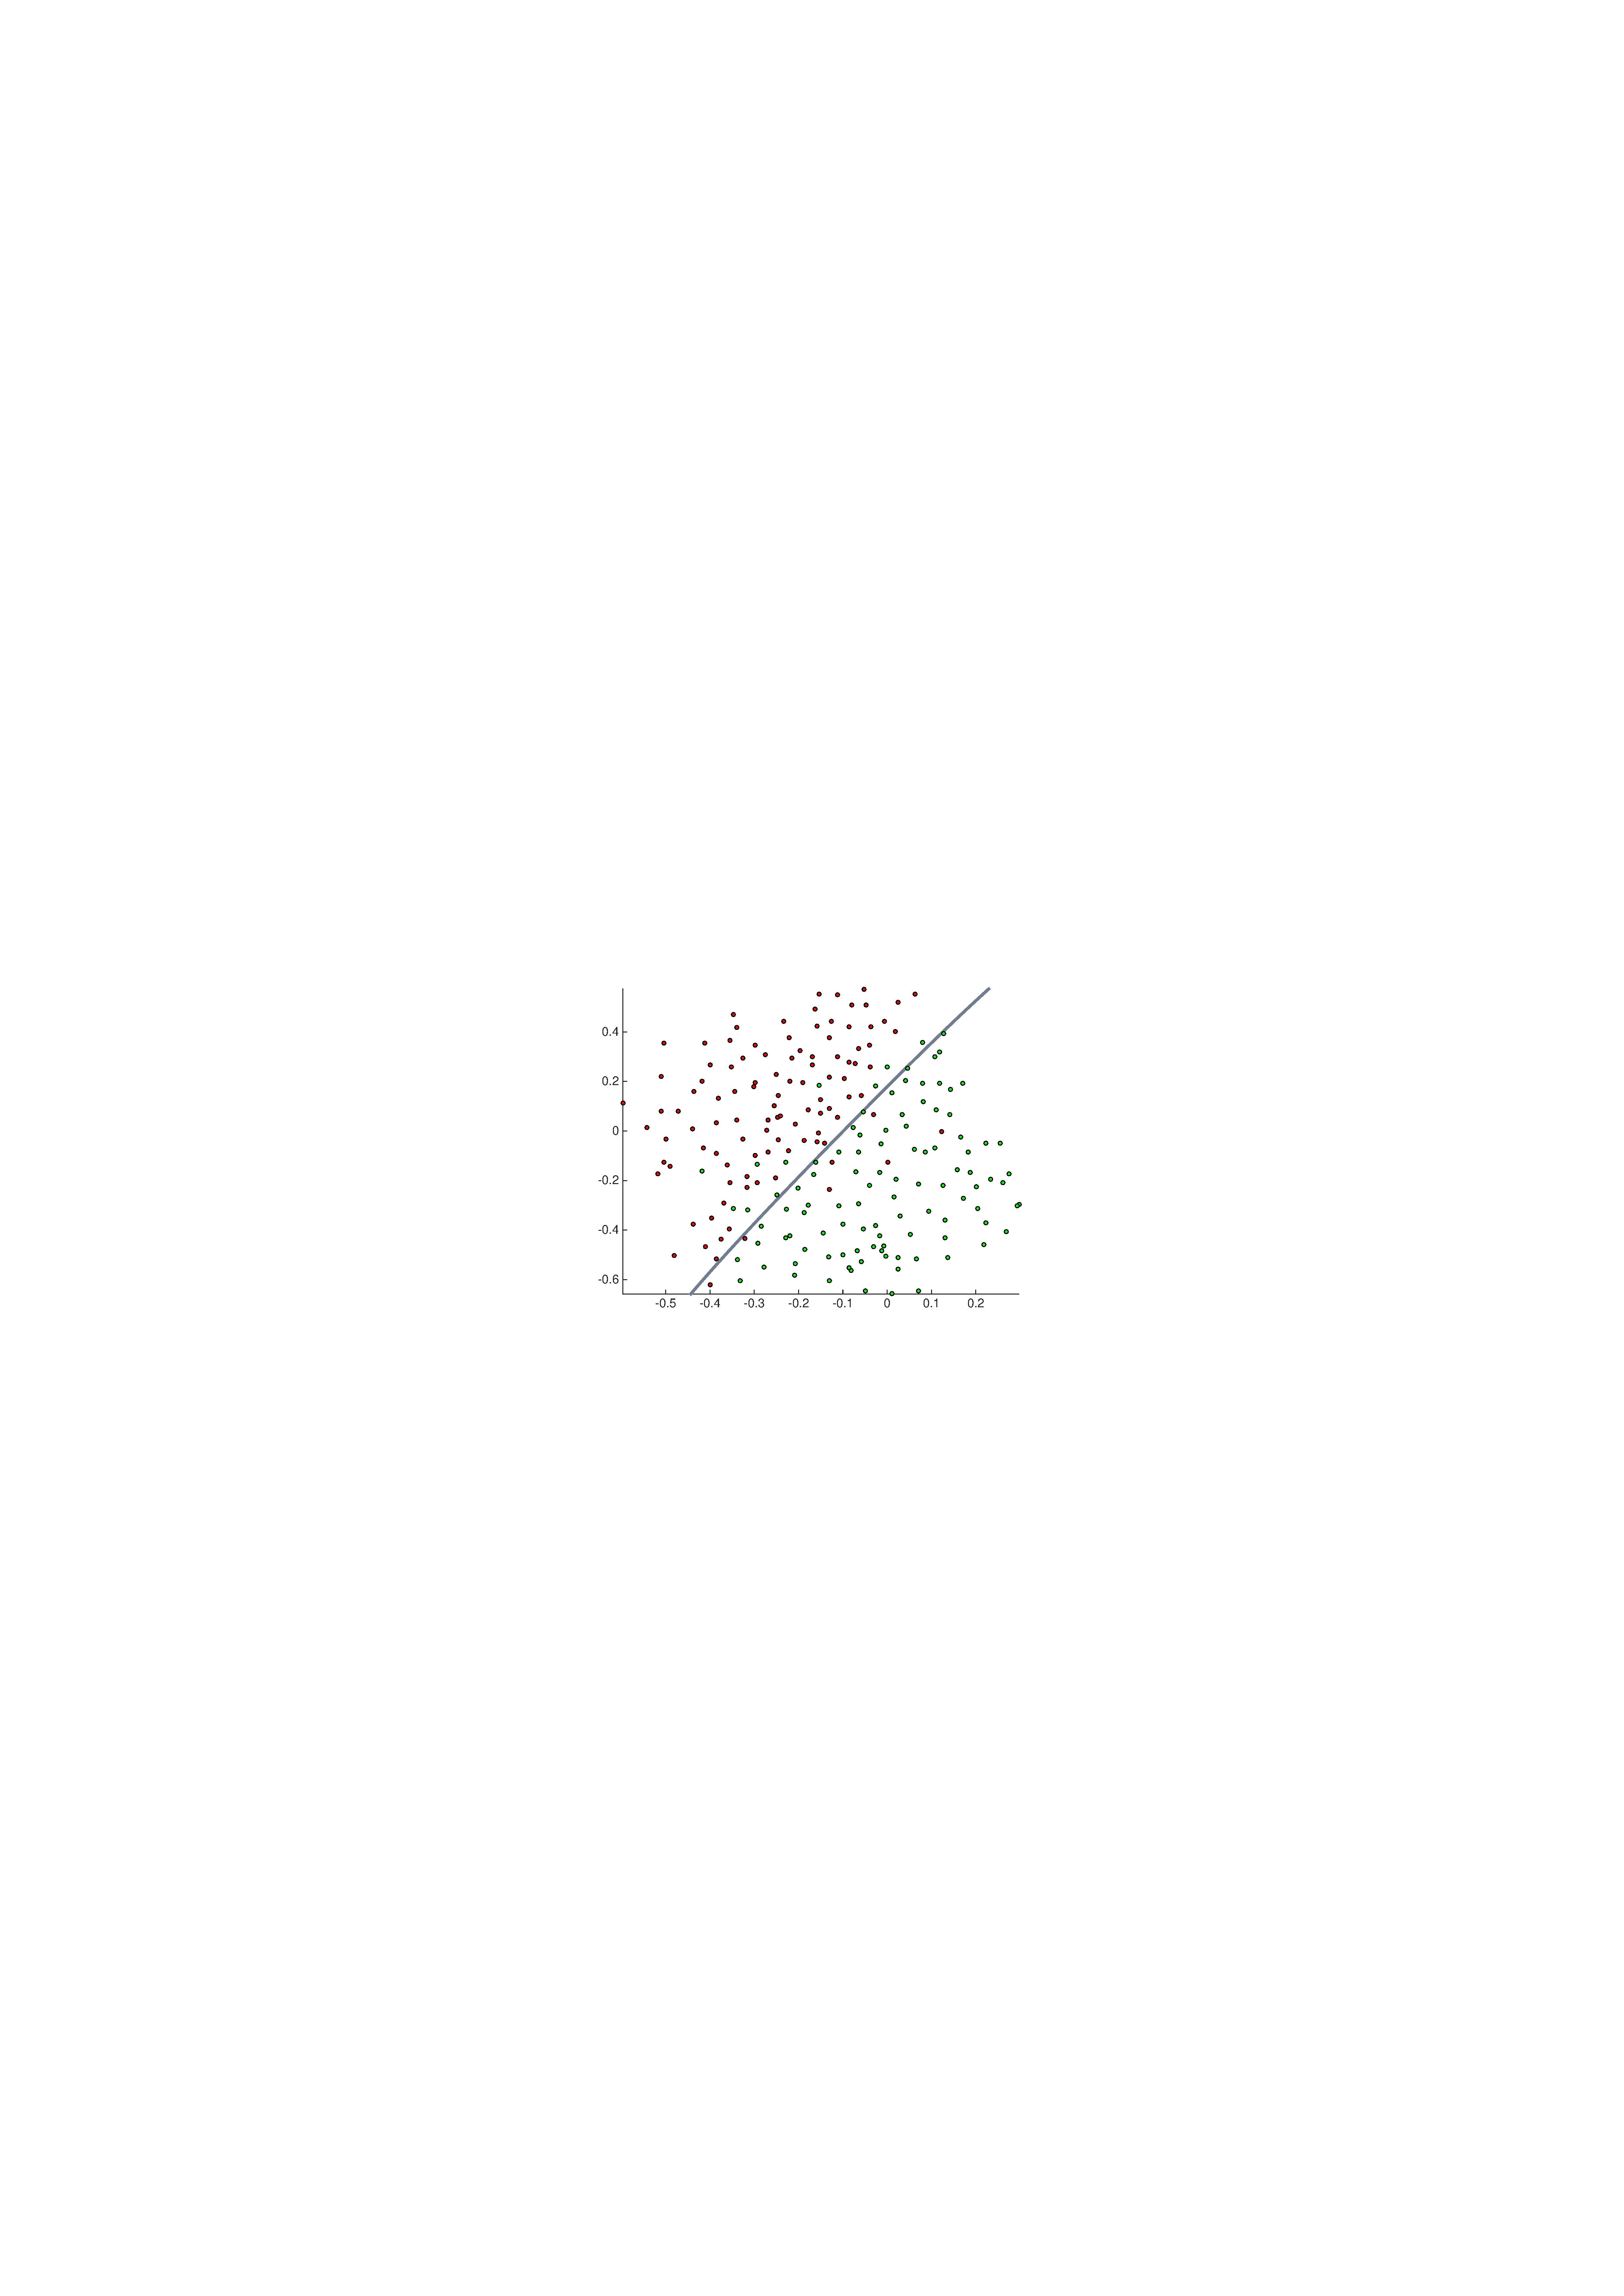
\includegraphics[width=.44\columnwidth]{gamma1}}
       \parbox{.45\columnwidth}{\center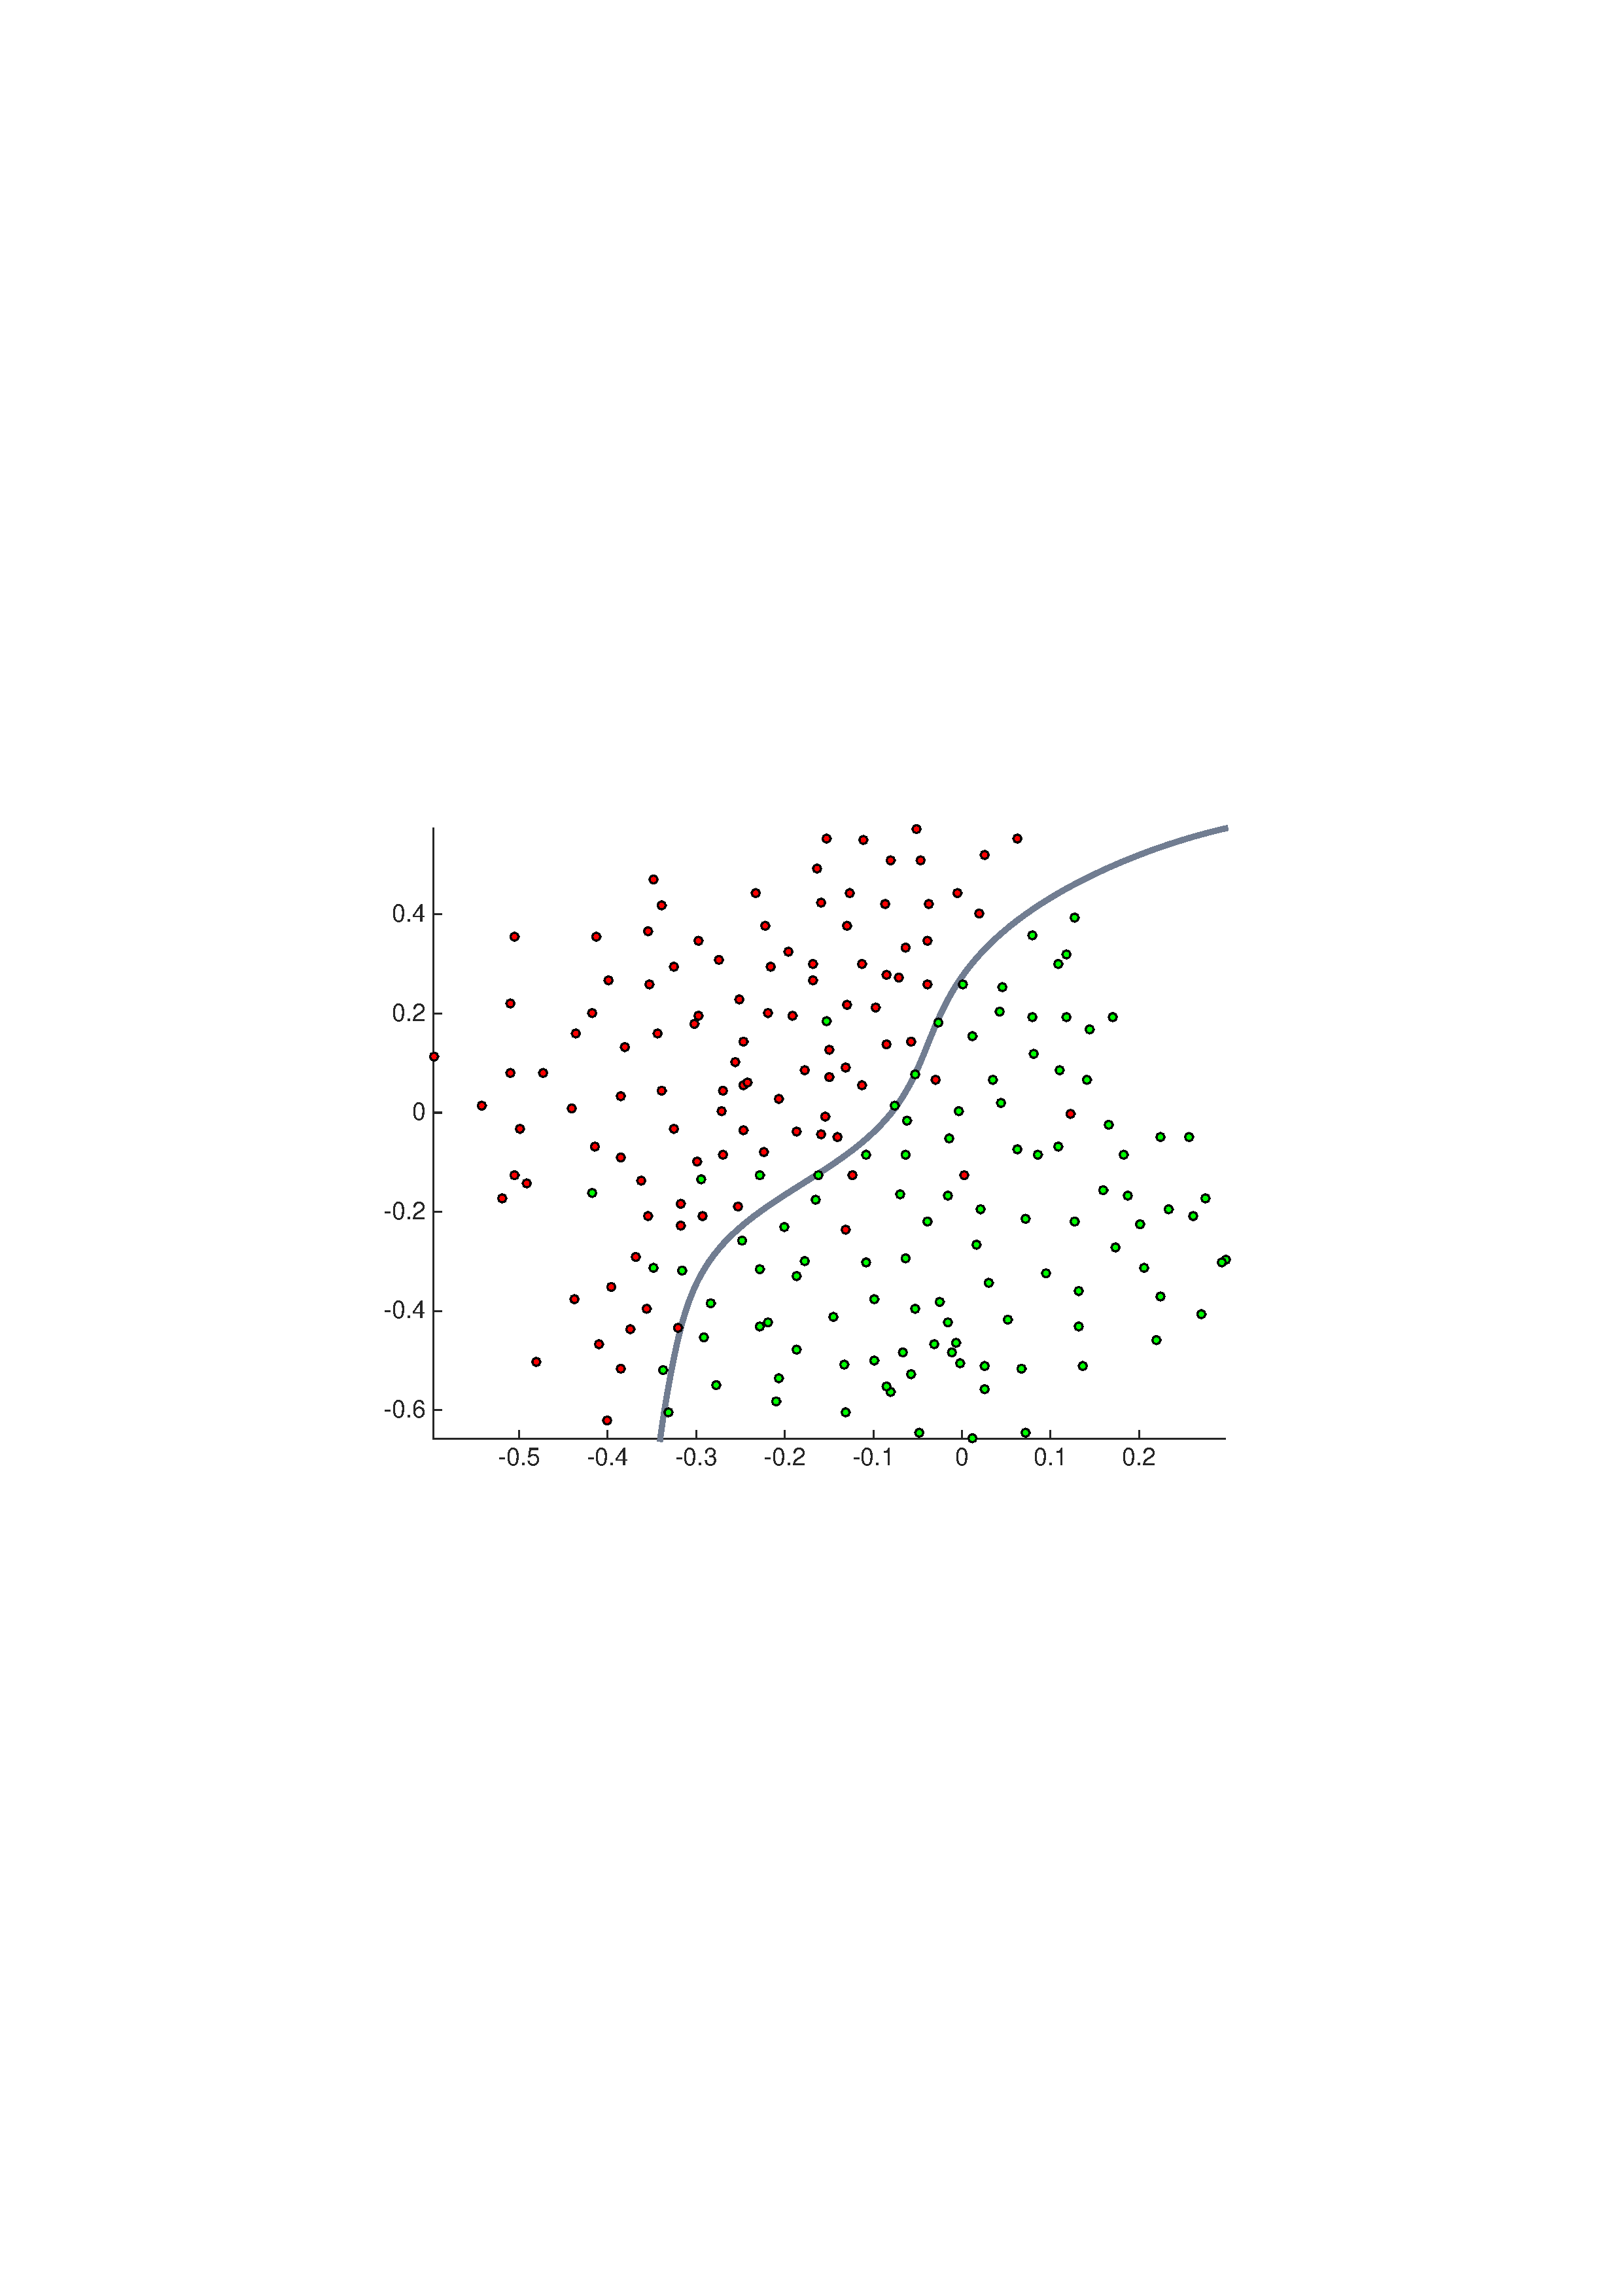
\includegraphics[width=.44\columnwidth]{gamma10}}
       \parbox{.45\columnwidth}{\center\scriptsize(a) $\gamma=1$}
       \parbox{.45\columnwidth}{\center\scriptsize(b) $\gamma=10$}
       \parbox{.45\columnwidth}{\center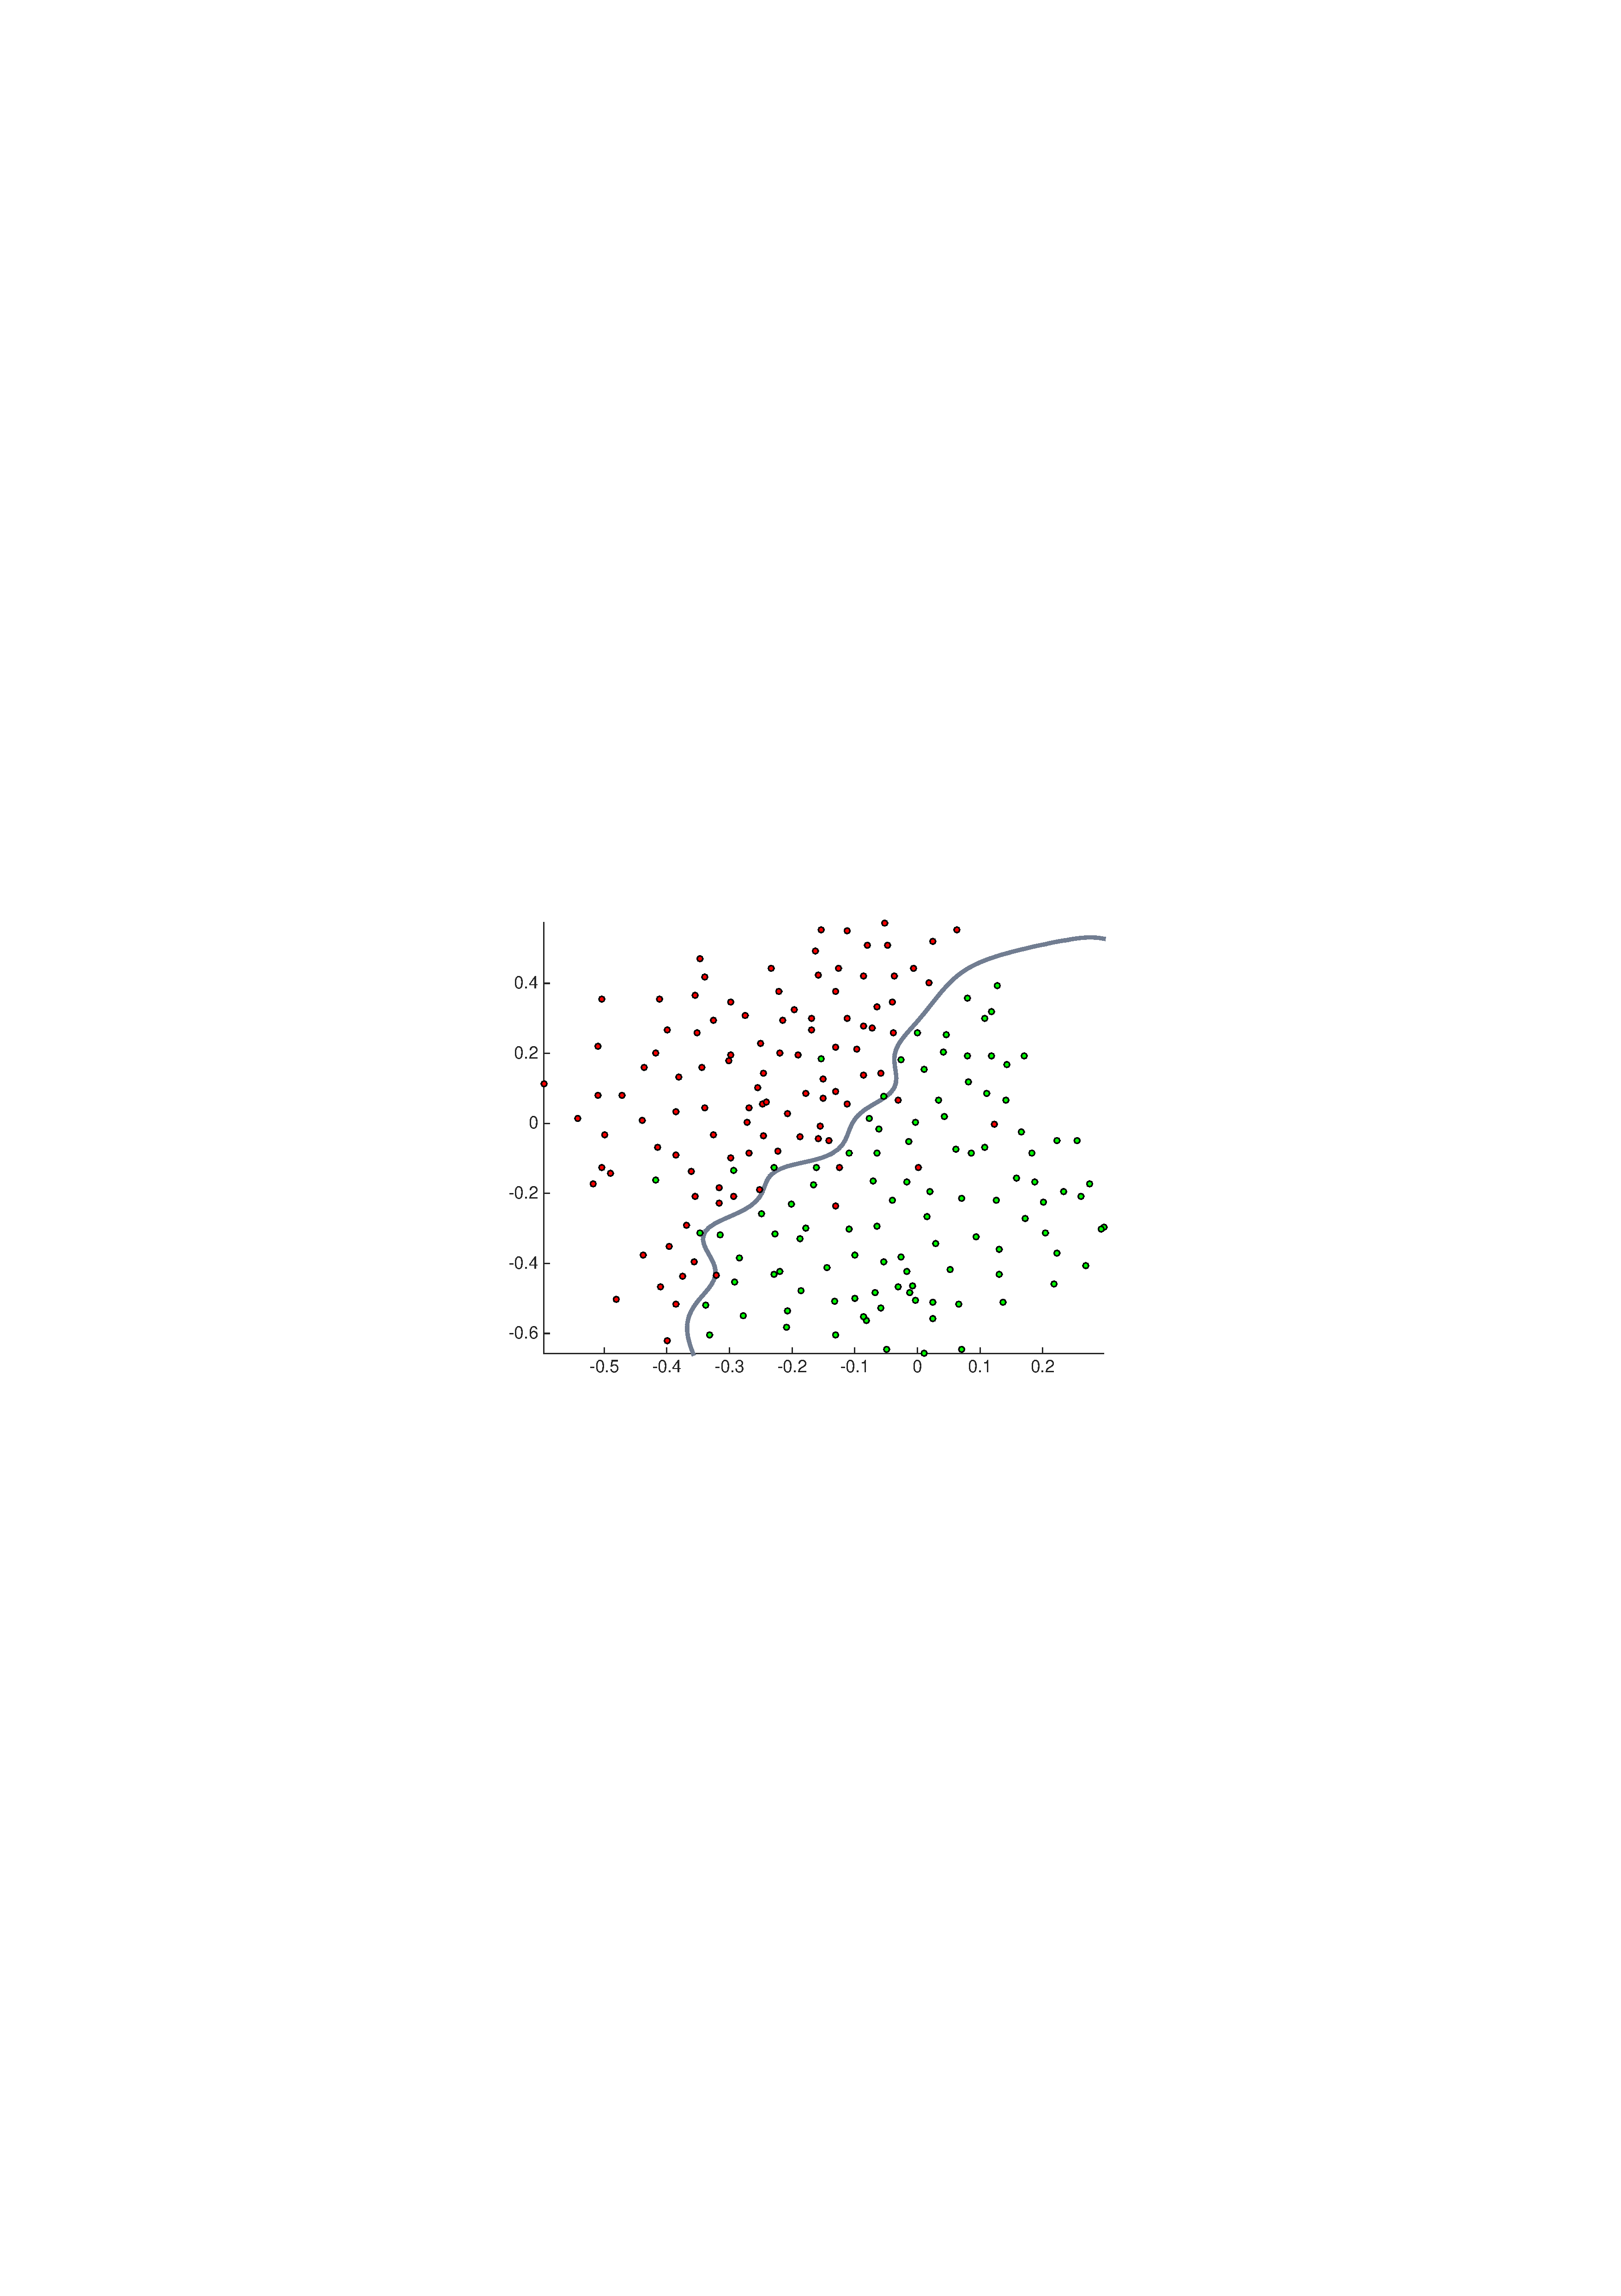
\includegraphics[width=.44\columnwidth]{gamma100}}
       \parbox{.45\columnwidth}{\center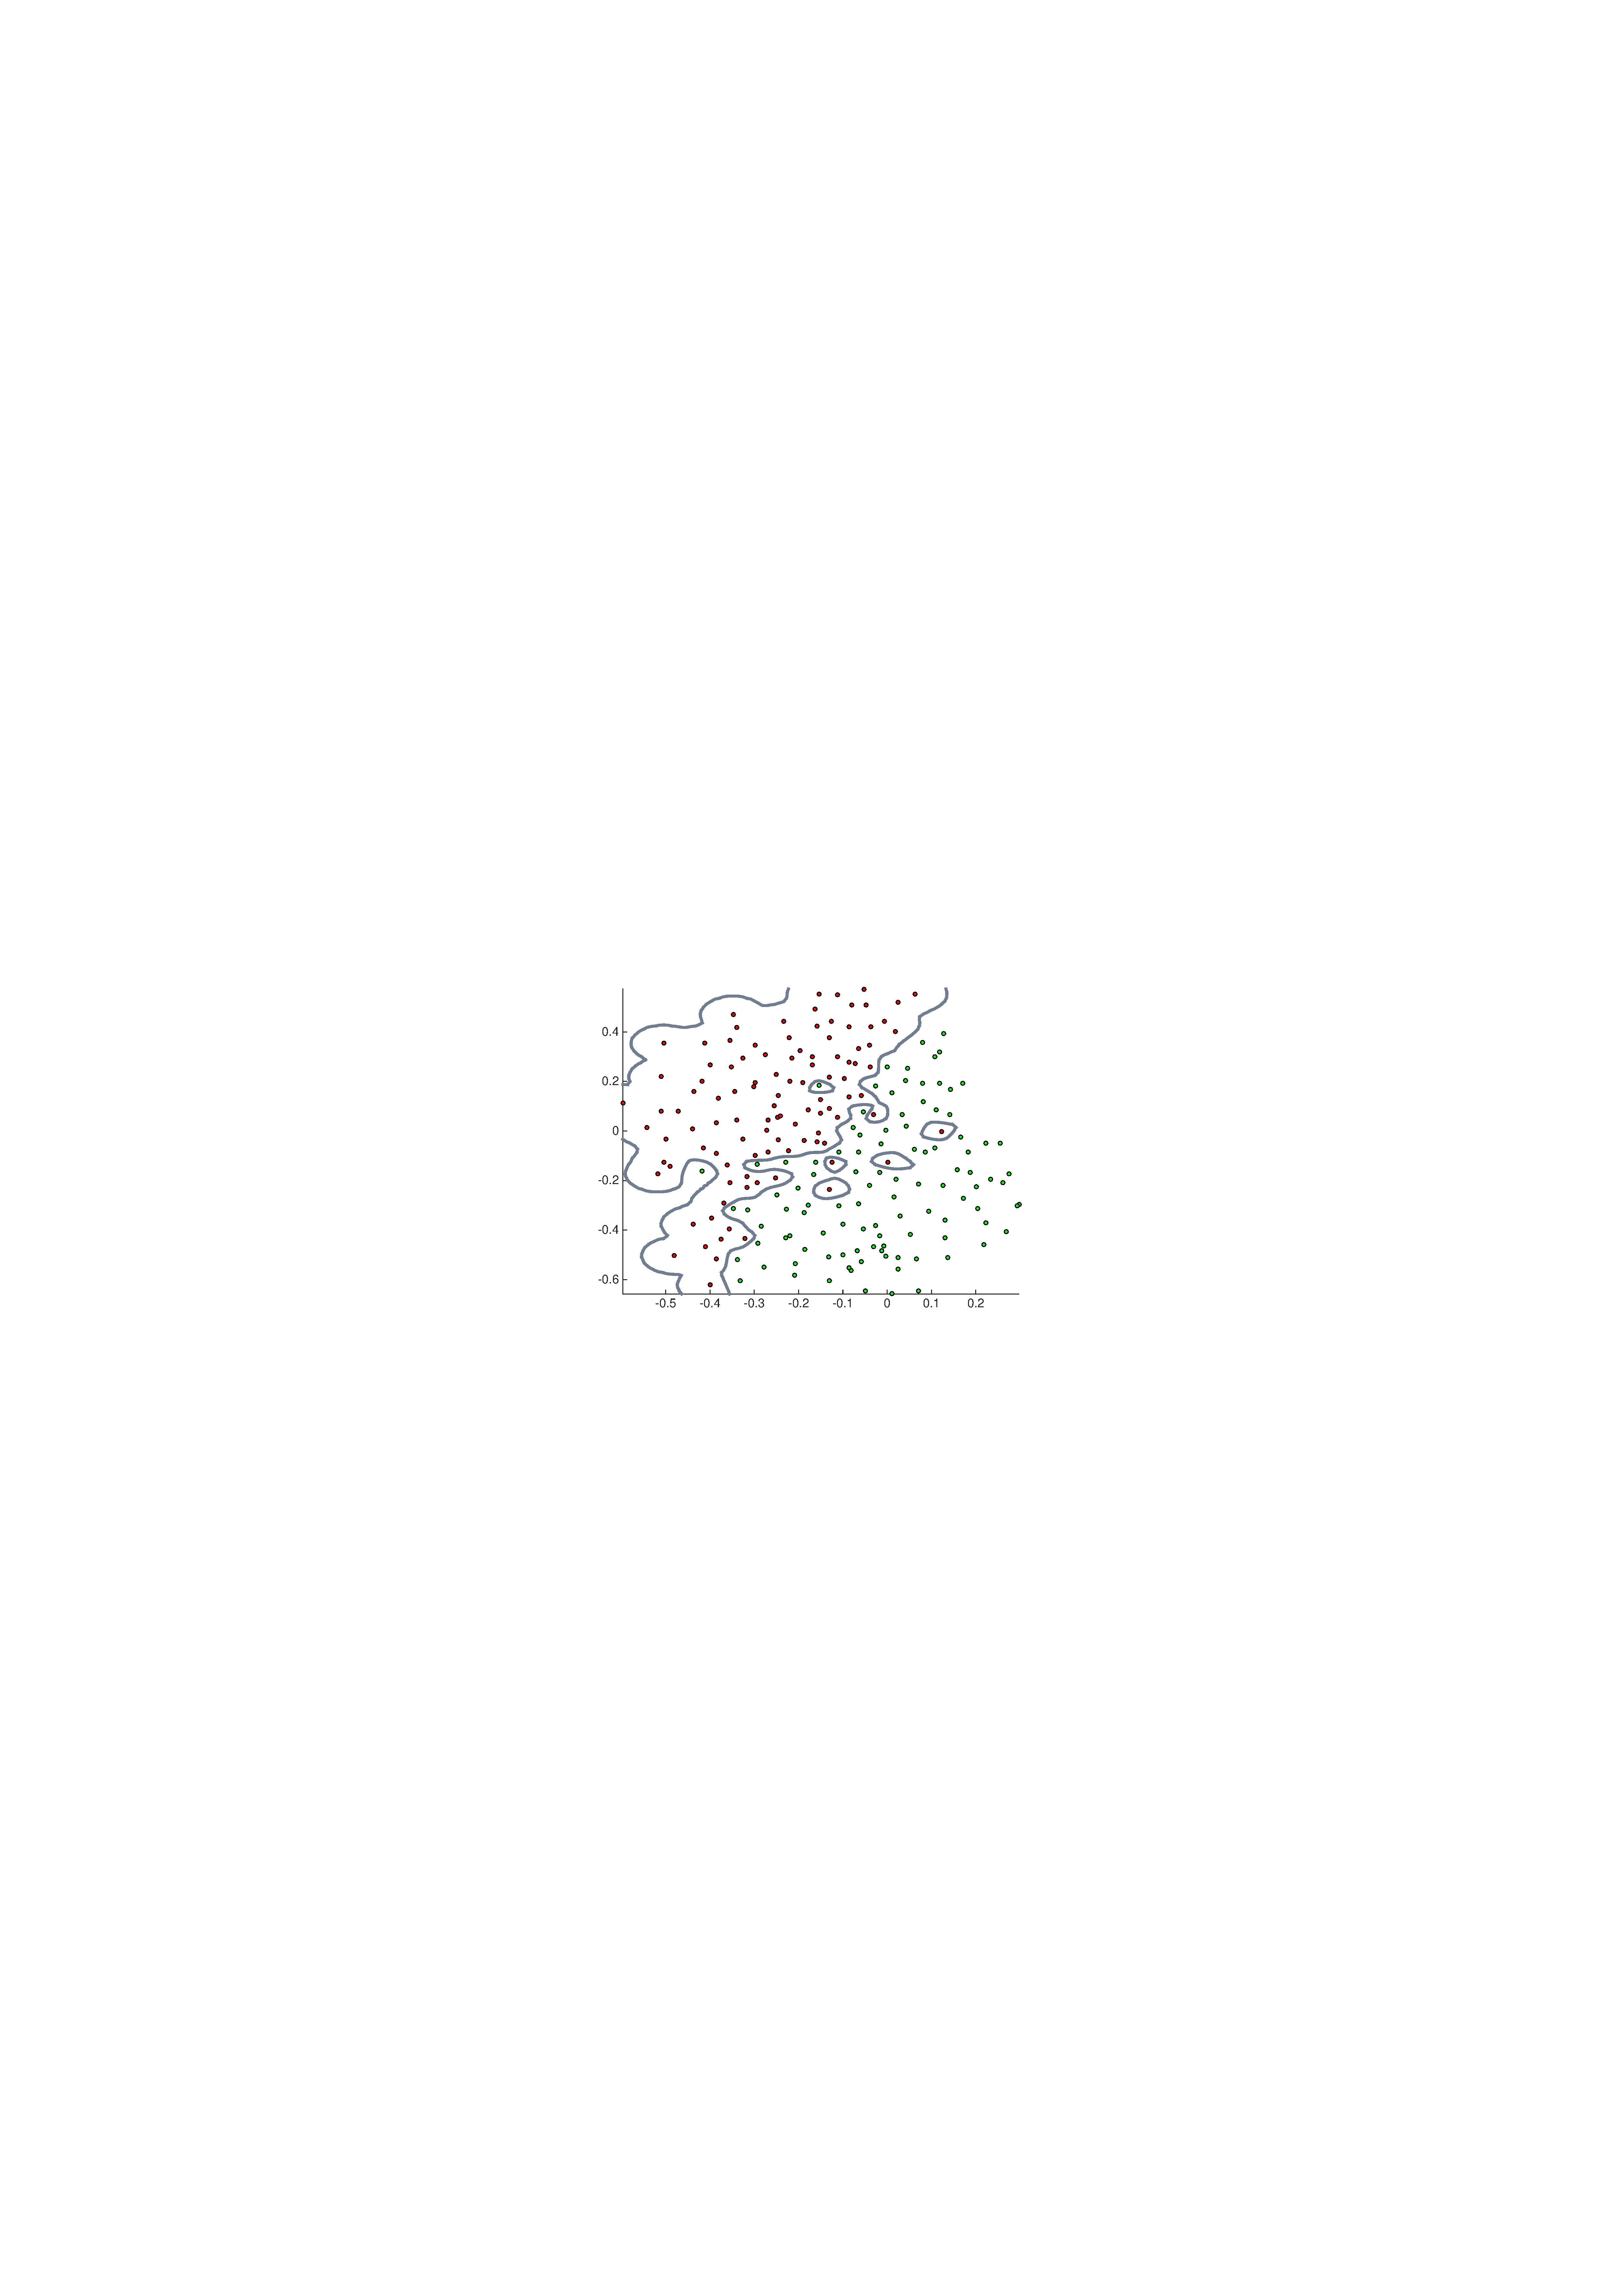
\includegraphics[width=.44\columnwidth]{gamma1000}}
       \parbox{.45\columnwidth}{\center\scriptsize(d) $\gamma=10$}
       \parbox{.45\columnwidth}{\center\scriptsize(e) $\gamma=1000$}
       \caption{SVM-based classification results under different $\gamma$'s}
       \label{fig:varvol}
       \end{center}
    \end{figure}
%
The classification accuracies on the training data for these models are 91.9\%, 93.3\%, 94.3\%, and 100\%, respectively. It is demonstrated that, with increasing $\lambda$, the classification boundary gets fitting to the training data, which results in higher classification accuracy, but with a sacrifice of overfitting.


\end{document}








  \end{lstlisting}
  %


